\chapter{Extrabilder}
\section{Zusammenbau der Hardware}\label{sec:BildliHardware}

\begin{figure}[h!]
	\centering
	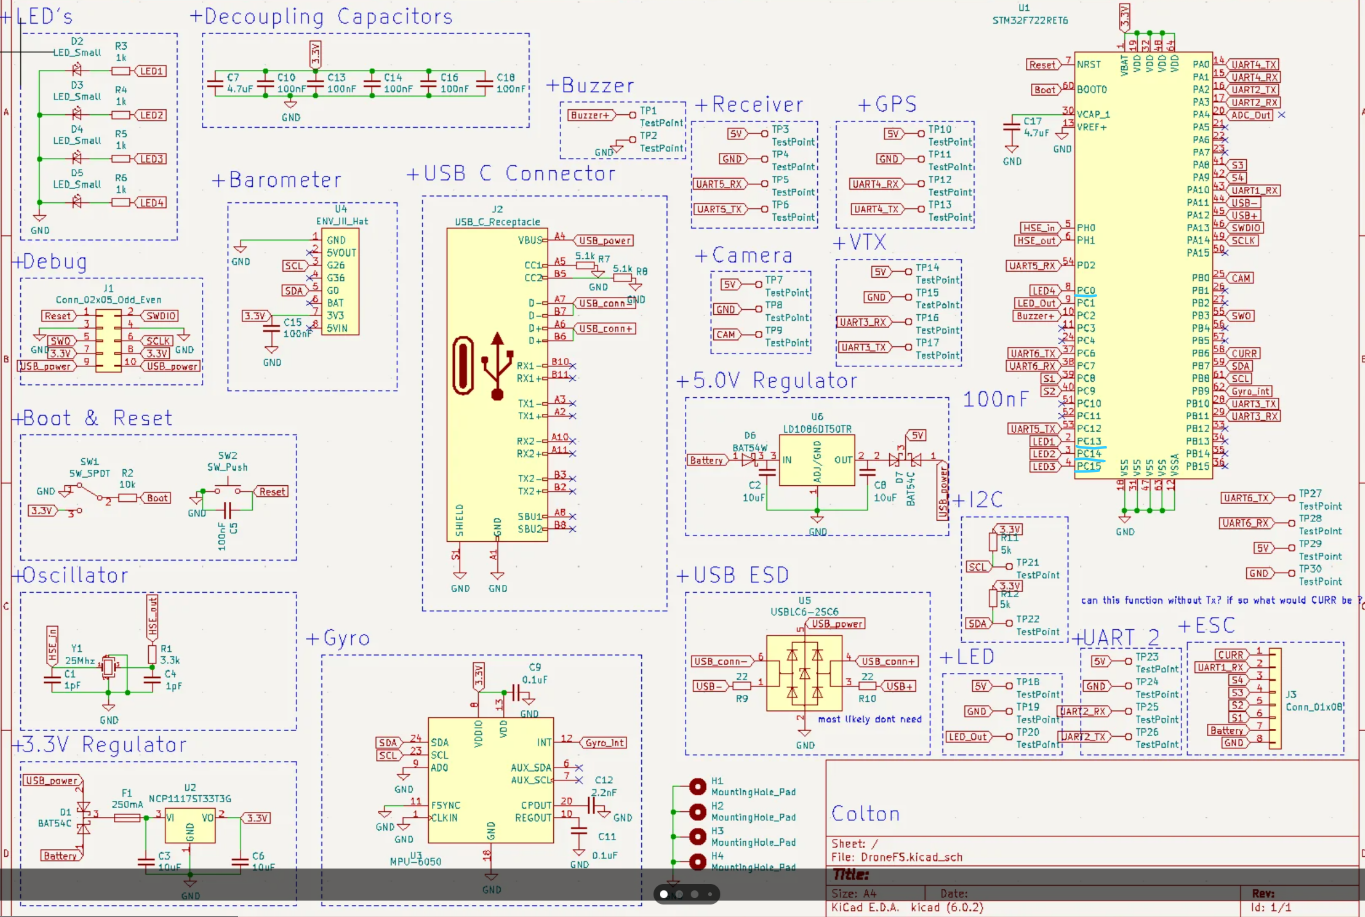
\includegraphics[height=0.3\textheight]{BoardOneNote.png}
	\caption{Schaltplan des Boards in OneNote.}
	\label{fig:boardonenote}
\end{figure}

\begin{figure}[h!]
	\centering
	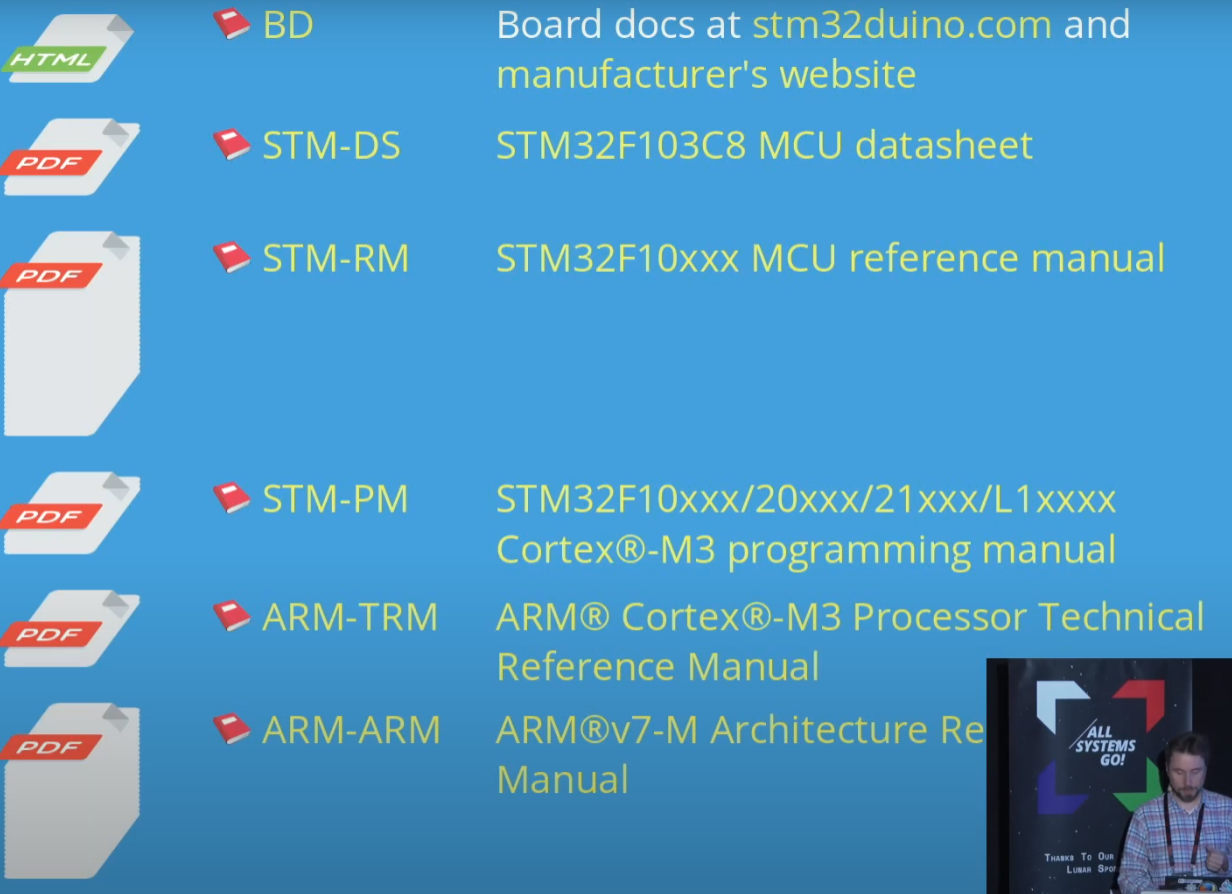
\includegraphics[height=0.3\textheight]{Docs.png}
	\caption{Screenshot von Dokumenten.}
	\label{fig:docs}
\end{figure}

\begin{figure}[h!]
	\centering
	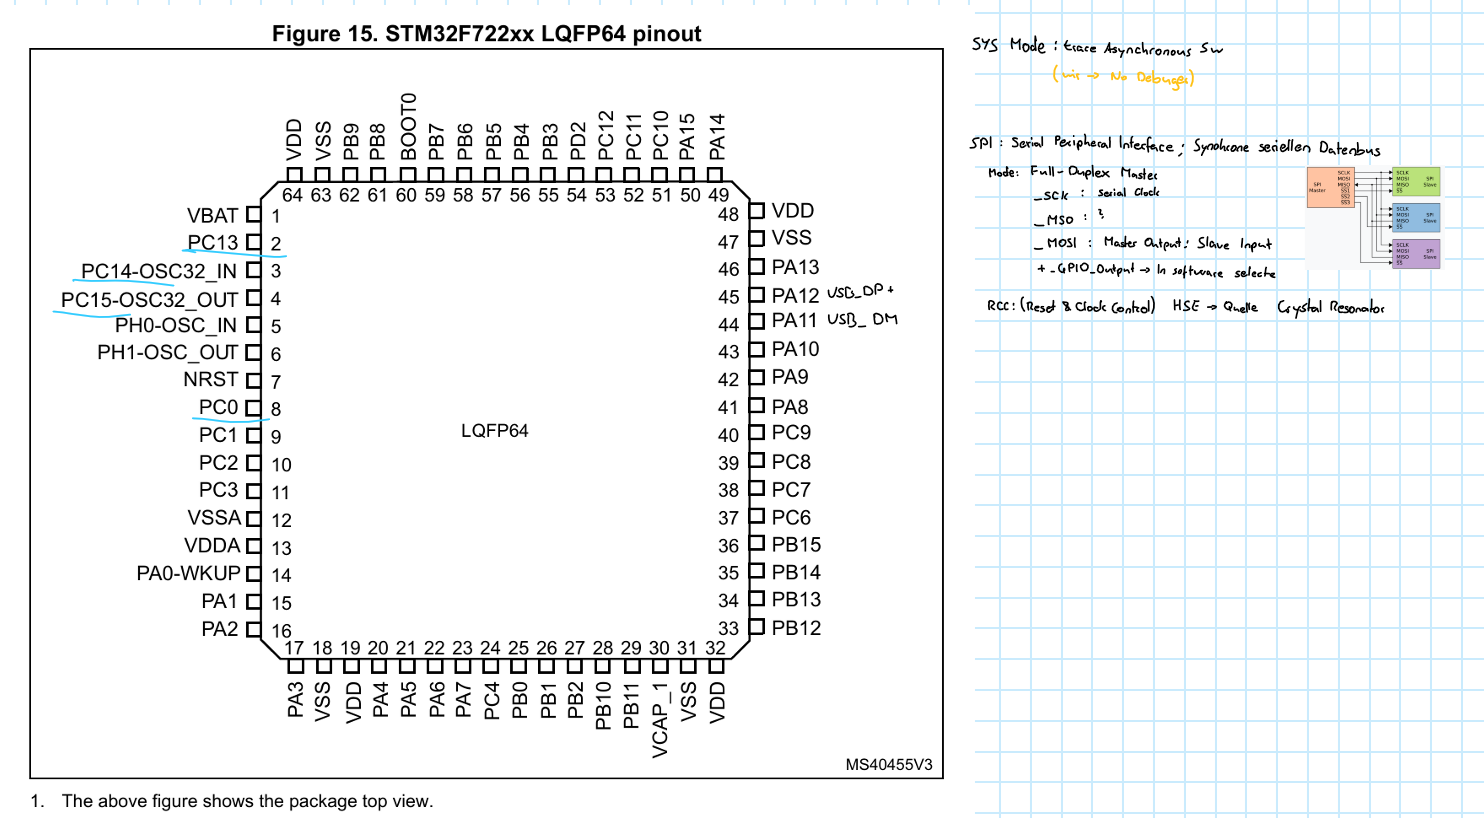
\includegraphics[height=0.3\textheight]{Figure15.png}
	\caption{Eine technische Abbildung (Figure 15).}
	\label{fig:figure15}
\end{figure}

\begin{figure}[h!]
	\centering
	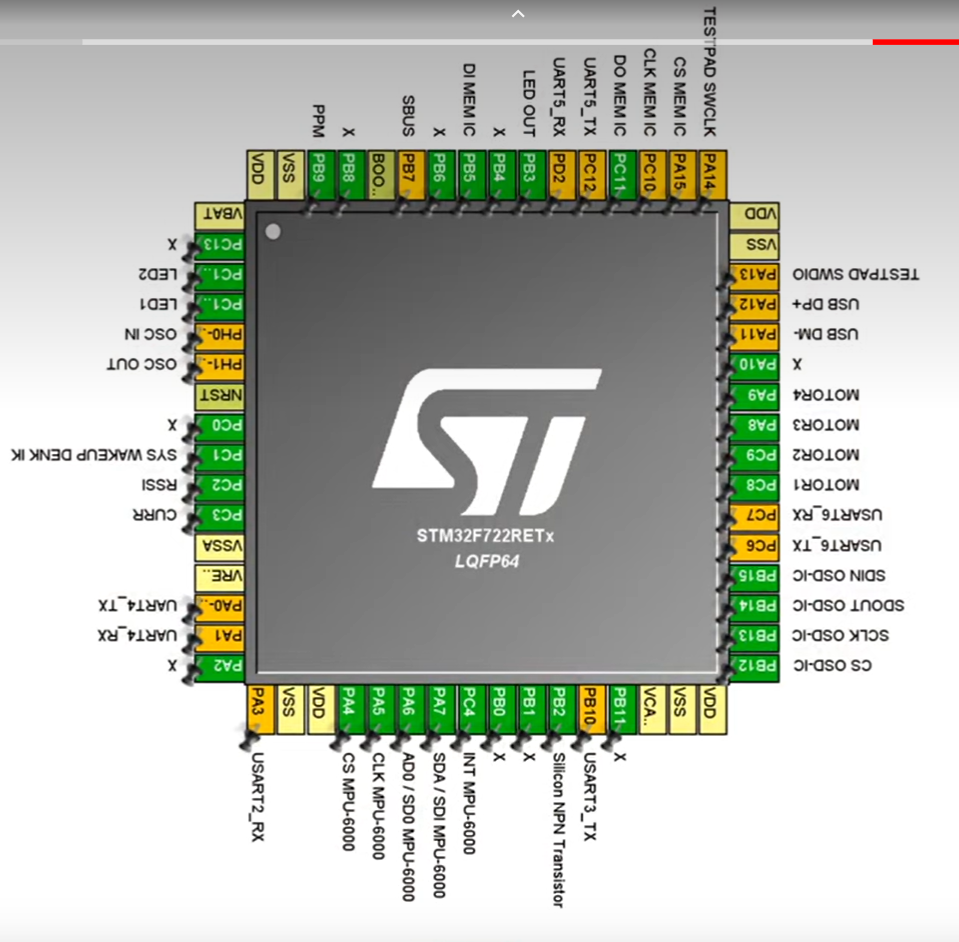
\includegraphics[height=0.3\textheight]{MambaF7.png}
	\caption{Mamba F7 Flight Controller.}
	\label{fig:mambaf7}
\end{figure}

\begin{figure}[h!]
	\centering
	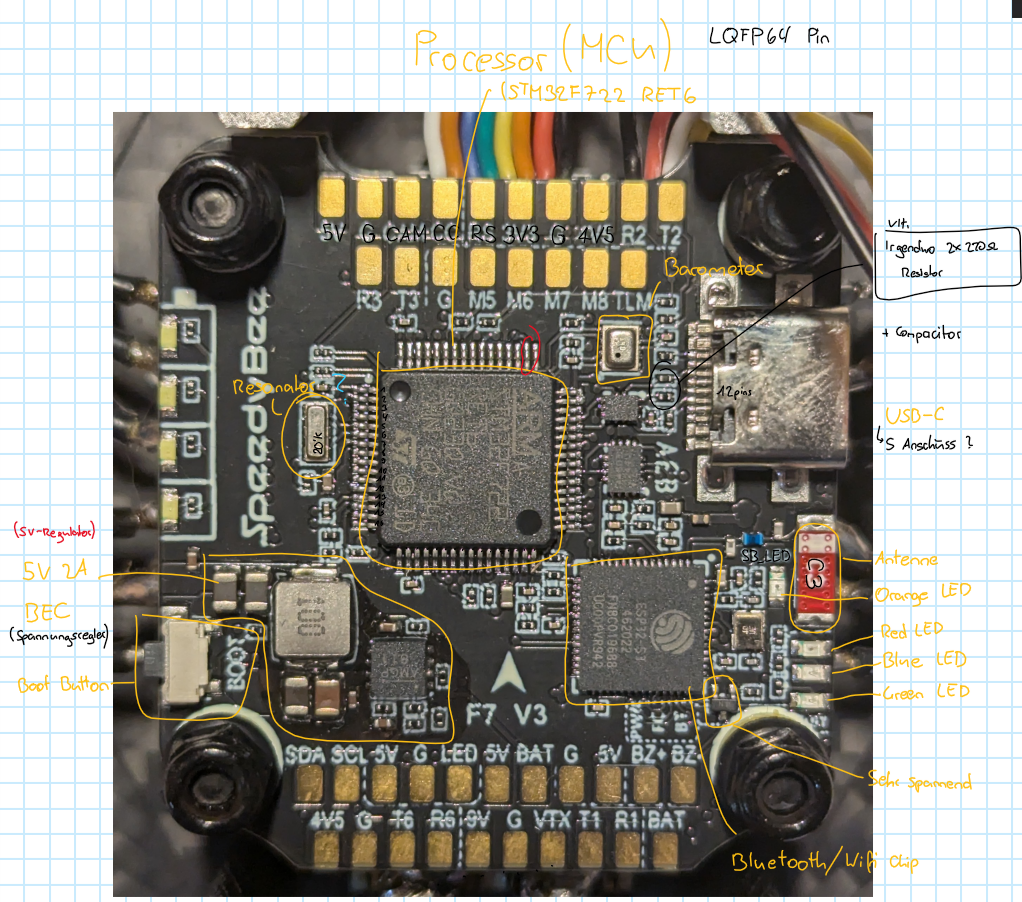
\includegraphics[height=0.3\textheight]{OneNote1.png}
	\caption{Schaltplan aus OneNote - Teil 1.}
	\label{fig:onenote1}
\end{figure}

\begin{figure}[h!]
	\centering
	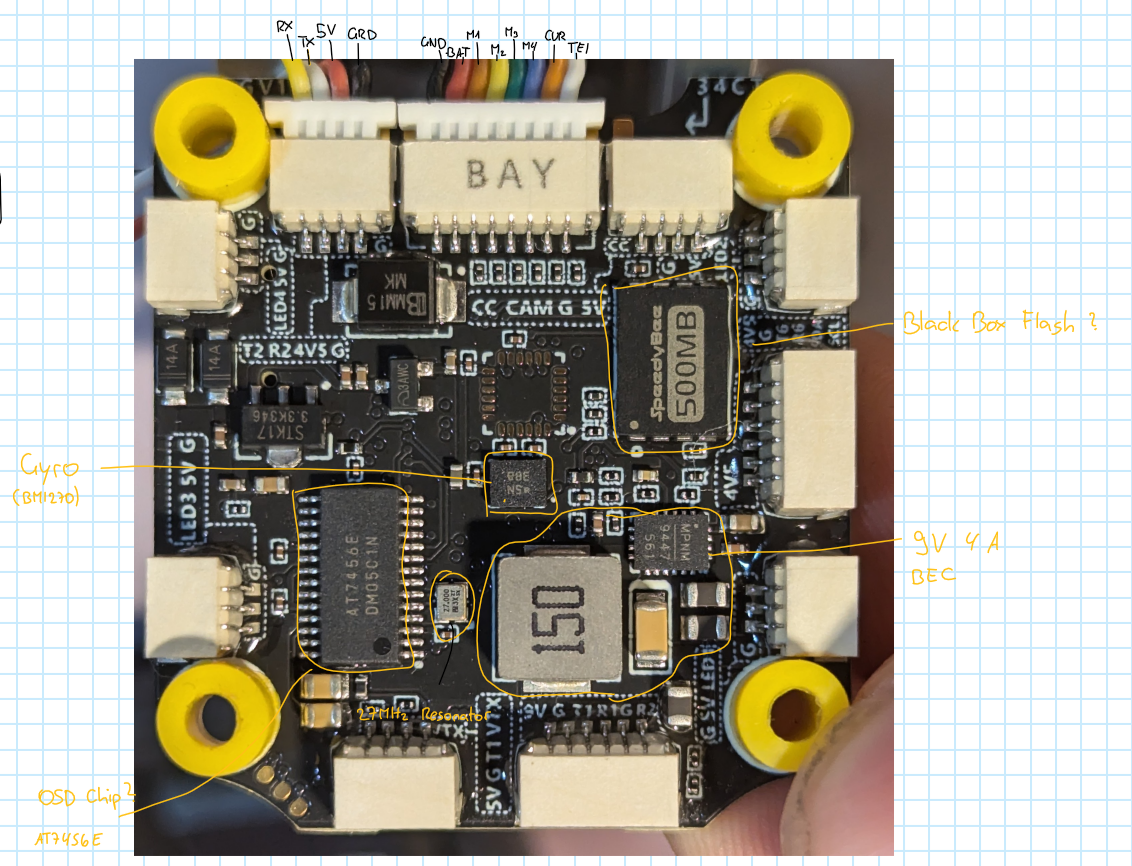
\includegraphics[height=0.3\textheight]{OneNote2.png}
	\caption{Schaltplan aus OneNote - Teil 2.}
	\label{fig:onenote2}
\end{figure}

\begin{figure}[h!]
	\centering
	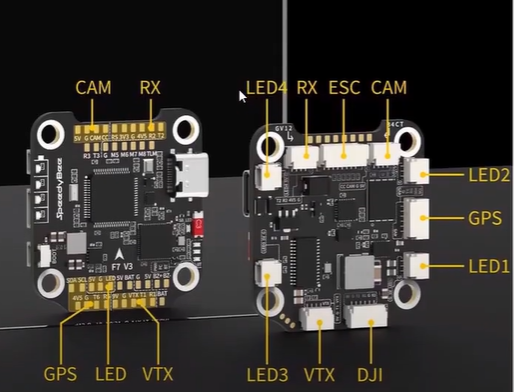
\includegraphics[height=0.3\textheight]{OneNote3.png}
	\caption{Schaltplan aus OneNote - Teil 3.}
	\label{fig:onenote3}
\end{figure}

\begin{figure}[h!]
	\centering
	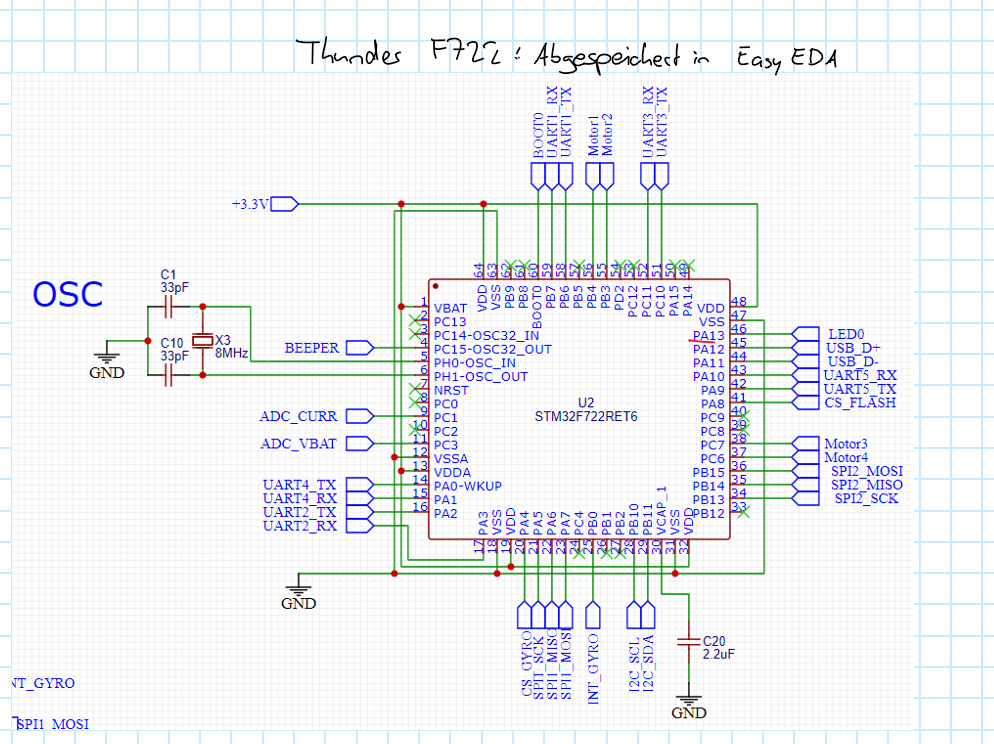
\includegraphics[height=0.3\textheight]{ThunderF722.png}
	\caption{Thunder F722 Schaltplan.}
	\label{fig:thunderf722}
\end{figure}

\begin{figure}[h!]
	\centering
	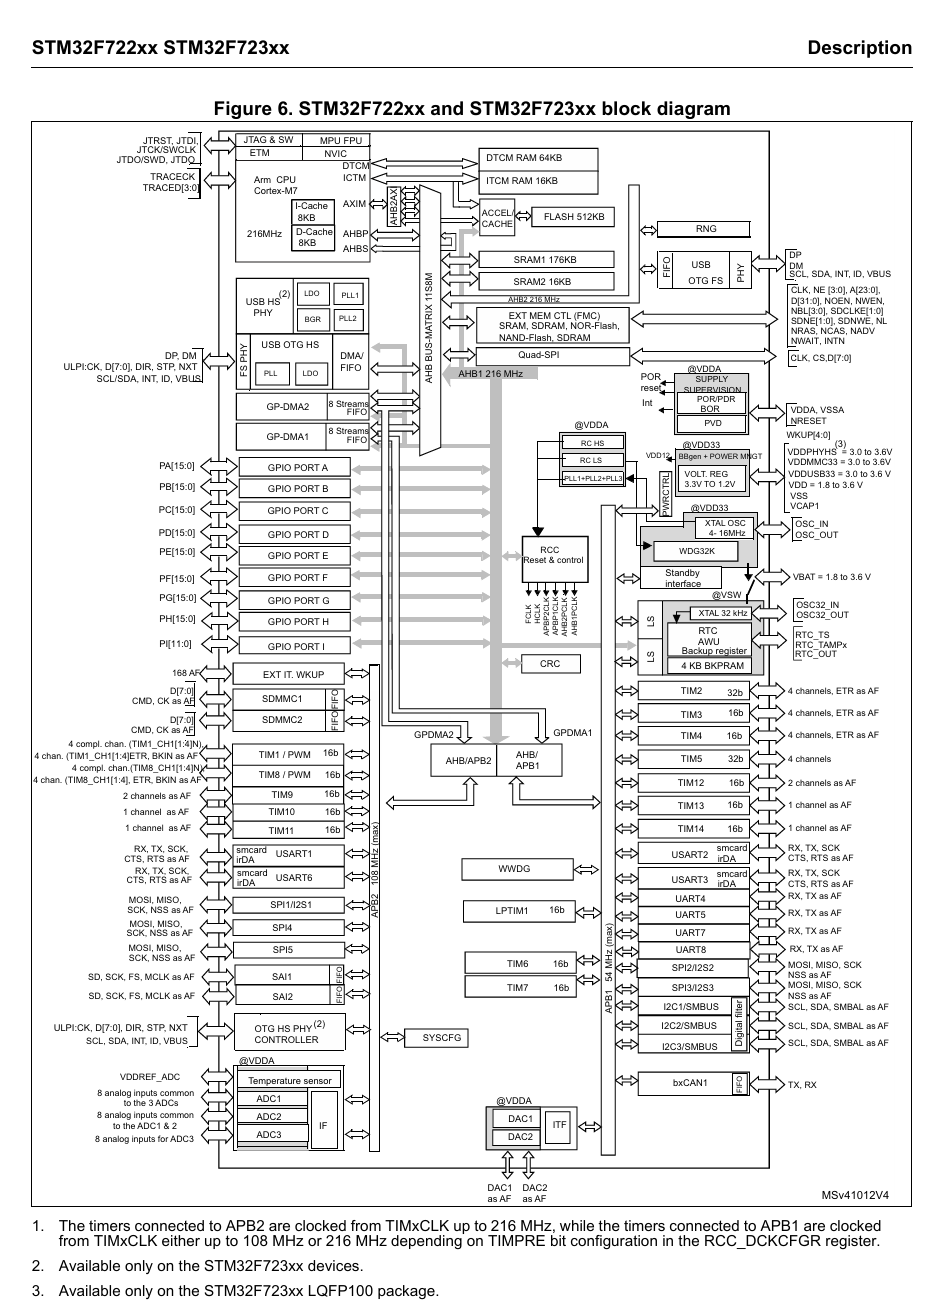
\includegraphics[height=0.5\textheight]{STM32F722xx.png}
	\caption{STM32F722xx Übersicht.}
	\label{fig:stm32f722xx}
\end{figure}
